
\begin{lemma}
A function f(x) is said to be convex if following inequality is true for $\lambda \in [0,1] :$  \label{opt/2/1/b/lemma1}
\begin{align}
    \lambda f(x_1) + (1-\lambda)f(x_2) \geq f(\lambda x_1 + (1-\lambda)x_2)
\end{align}
\end{lemma}
Given :
\begin{align}
    \brak{x-1}^2+3,x \in \sbrak{-3,1} , x \in \sbrak{-3,1}
\end{align}
Checking convexity of $f(x)$ :
\begin{equation}
\begin{aligned}
    &\lambda\brak{\brak{x_1-1}^2+3} + (1-\lambda)\brak{\brak{x_2-1}^2+3} \geq \\
    &\brak{\brak{\lambda x_1 + (1-\lambda)x_2}-1}^2 +3
\end{aligned}
\end{equation}
resulting in
\begin{align}
    x_1^2\brak{\lambda-\lambda^2}+x_2^2\brak{{\lambda-\lambda^2}}- 2x_1x_2\brak{{\lambda-\lambda^2}} &\geq 0 \\
    \implies \brak{\lambda-\lambda^2}\brak{x_1^2+x_2^2-2x_1x_2} &\geq 0 \\
    \implies \lambda\brak{1-\lambda}\brak{x_1-x_2}^2 &\geq 0 
\end{align}
Hence,using lemma \ref{opt/2/1/b/lemma1}, given $f(x)$ is a convex function .
\begin{enumerate}
    \item For Maxima : \\
    Using gradient ascent method,
    \begin{align}
        x_{n+1} &= x_n + \alpha \nabla f(x_n) \\
        \implies x_{n+1} &= x_n + \alpha \brak{2x_n-2}
    \end{align}
    
    Taking $x_0=-3,\alpha=0.001$ and precision= \\ 0.00000001,values obtained using python are:
    \begin{align}
        \boxed{\text{Maxima} = 18.999999999940298 \approx 19 }\\
        \boxed{\text{Maxima Point} = -2.9999900126845568 \approx -3}
    \end{align}
    
    
    \begin{figure}[!ht]
    \centering
    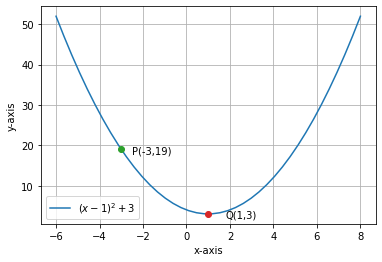
\includegraphics[width=\columnwidth]{solutions/su2021/2/1/b/Figure/Figure.png}
    \caption{$f(x)=\brak{x-1}^2+3$}
    \label{opt/2/1/b/f(x)}	
    \end{figure}
    \item For Minima : \\
    
    \numberwithin{table}{section}
    \begin{table}[!ht]
    \centering
    \begin{tabular}{|c|c|} 
    \hline
    $x$ & $f(x)$ \\
    \hline
    -3& 19 \\
    \hline
   1 & 3 \\
    \hline
    \end{tabular}
    \caption{Value of $f(x)$}
    \label{opt/2/1/b/tab:table1}
    \end{table}
    
    Critical point is given by
    \begin{align}
        \nabla f(x) &= 0 \\
        \implies x &= 1
    \end{align}
    
    and,end points are $x=-3$ and $x=1$ .
    
    Using table \ref{opt/2/1/b/tab:table1},
    \begin{align}
        \boxed{\text{Minima} = 3}\\
        \boxed{\text{Minima Point} = 1}
    \end{align}
    
\end{enumerate}

